\documentclass[11pt,a4paper]{article}

\usepackage[margin=1in]{geometry}
\usepackage{graphicx}
\usepackage{booktabs}
\usepackage{amsmath,amssymb}
\usepackage[hidelinks]{hyperref}
\usepackage{natbib}
\usepackage{float}

\title{Schedule-Free On-Demand Water Transport in Bergen:\\ Progress Report}
\author{}
\date{\today}

\begin{document}

\maketitle

\begin{abstract}
\noindent
This note documents the progress made so far on a project that designs the real-time dispatch logic for a small-boat, on-demand water transport service in Bergen, Norway. The service does not exist yet: rather than optimizing an existing system, the project builds a model of how such a service would operate, replacing fixed timetables with a dispatch policy that recomputes itself every few minutes. Three pieces are covered in this report: a navigable routing module that computes real, coastline-respecting travel times between the four candidate stops (replacing an earlier straight-line approximation); a synthetic demand model anchored in official Norwegian population and employment data; and a first, deliberately simple simulation environment, implemented to the Gymnasium interface standard, that will host the dispatch policy. This is a partial, working progress report: the dispatch policy itself, its verification, and the resulting metrics are still under review and are intentionally left out of this version.
\end{abstract}

\tableofcontents
\newpage

% =====================================================================
\section{Introduction and Motivation}
% =====================================================================

Bergen is a coastal city whose public transport network is structured as a hub-and-spoke system centered on the city center, a layout imposed by the surrounding fjords and mountains. As the city grows and tourism increases, this network is under increasing pressure, and land-based expansion is constrained by the same geography that makes it congested in the first place. The fjords that divide the city are, at the same time, an underused transport corridor.

This project explores a small-boat, on-demand water transport service as a complementary mode. Two principles guide its design. First, the service is not modeled as a profit-making venture (public transport of this kind is rarely self-financing, and its justification is environmental and related to congestion relief, not revenue); the objective is to deliver a good level of service efficiently, not to maximize income. Second, the flexible layer of the service has no fixed timetable: a passenger requests a trip and a boat is dispatched to serve it, subject to a waiting-time guarantee, and the dispatch policy is recomputed at short, regular intervals rather than following a pre-published schedule. Section 2 situates this "schedule-free" operating philosophy, and the static water-taxi model it builds on, within the closely related literature.

\paragraph{Scope of this report.} This is a progress note, not a finished piece of work. It covers the routing and demand modeling that feed the project (Sections 3 and 4) and a first version of the simulation environment (Section 5). The environment described here is intentionally simple: it is a first iteration meant to establish a working structure, not the final model the project targets. The dispatch policy that will control it, its verification, and the resulting metrics are still being reviewed internally and are left out of this version deliberately.

% =====================================================================
\section{Related Work}
% =====================================================================

Three papers anchor the modeling choices described in this report.

\citet{Gu2021} formulate a static location, fleet-sizing, and routing model for a water-taxi system connecting the same four stops used in this project (Kleppestø, Laksevåg, Bryggen, and Sandviken). It is the closest precedent in terms of the physical instance, and it is used in Section 4 as one reference point for the scale of daily demand.

\citet{Braathen2024} study autonomous ferry scheduling under labor regulations, comparing autonomous and manually operated fleets. The demand-generation approach in Section 4 is adapted from their multiplicative, gravity-style formulation, and the group-size statistics they report are used to calibrate the group-size distribution used here.

\citet{SanchezMartinez2017} develop a schedule-free operating paradigm for high-frequency transit control. Their central point, that abandoning fixed schedules in favor of real-time, resource-aware control can improve service quality provided the underlying control problem can be solved effectively, is the conceptual starting point for treating dispatch in this project as a control problem rather than a scheduling problem.

% =====================================================================
\section{Navigable Routing}
% =====================================================================

Travel times between the four stops are computed from a navigable-routing module rather than from straight-line (Haversine) distances. An earlier, straight-line version of the travel-time matrix was found, on visual inspection, to draw lines that cross land near Bryggen, which sits inside the Vågen bay next to the Nordnes peninsula (straight-line distances are therefore not usable directly and are corrected here).

\paragraph{Water/land classification.} A basemap tile mosaic covering the four stops is downloaded at zoom level 14, which corresponds to a fixed Web Mercator resolution of $156543.03392 / 2^{14} \approx 9.55$ m/pixel. Because Web Mercator distorts distances by a factor of $1/\cos(\text{latitude})$, and Bergen sits at approximately $60.4^{\circ}$N, the real ground resolution is $9.55 \times \cos(60.4^{\circ}) \approx 4.7$ m/pixel. Each pixel is classified as water or land by its Euclidean distance, in RGB space, to a reference water color sampled from the basemap style (threshold of 15 color units); the resulting mask is pixel-for-pixel aligned with the source map, since both are produced by the same Web Mercator projection formula and the same Earth radius.

\paragraph{Graph and shortest paths.} Each water pixel becomes a node in an 8-connected graph (4 orthogonal and 4 diagonal neighbors), with edge weights equal to the real distance between pixel centers; land pixels are simply absent from the graph, so no edge can cross land. The four stops are snapped to the nearest water pixel, restricted to the graph's main connected component, to avoid anchoring a stop to an isolated puddle unconnected to open water. A multi-source Dijkstra search (\texttt{scipy.sparse.csgraph.dijkstra}) then computes the shortest navigable path between every pair of stops in a single call, exact because all edge weights are non-negative real distances.

\paragraph{Design speed and resulting matrix.} Rather than calibrating vessel speed against an existing ferry line, a fixed design speed of 30 km/h ($\approx 16.2$ knots) is used for the whole fleet, treated as a design decision for the small on-demand vessels rather than an empirical calibration. Table~\ref{tab:matriz-tiempos} reports the resulting travel-time matrix, and Table~\ref{tab:comparacion-rutas} compares it against the straight-line matrix it replaces: routing around land adds between 6\% and 24\% to travel distance depending on the pair, with Laksevåg (whose corrected location sits further inside the Puddefjorden) showing the largest correction because the detour around the Nordnes peninsula is large relative to its own distance to the other stops.

\begin{table}[H]
\centering
\caption{Navigable travel-time matrix (minutes), 30 km/h design speed.}
\label{tab:matriz-tiempos}
\begin{tabular}{lrrrr}
\toprule
 & Kleppestø & Laksevåg & Bryggen & Sandviken \\
\midrule
Kleppestø & - & 5.3 & 11.5 & 9.6 \\
Laksevåg  & 5.3 & - & 8.6 & 8.6 \\
Bryggen   & 11.5 & 8.6 & - & 6.8 \\
Sandviken & 9.6 & 8.6 & 6.8 & - \\
\bottomrule
\end{tabular}
\end{table}

\begin{table}[H]
\centering
\caption{Straight-line vs. navigable travel times, all six stop pairs.}
\label{tab:comparacion-rutas}
\begin{tabular}{lrrr}
\toprule
Pair & Straight-line (min) & Navigable (min) & Difference \\
\midrule
Laksevåg $\leftrightarrow$ Bryggen   & 7.0  & 8.6  & +23.8\% \\
Kleppestø $\leftrightarrow$ Sandviken & 8.7  & 9.6  & +10.5\% \\
Bryggen $\leftrightarrow$ Sandviken   & 6.3  & 6.8  & +8.9\% \\
Kleppestø $\leftrightarrow$ Laksevåg  & 4.9  & 5.3  & +7.8\% \\
Kleppestø $\leftrightarrow$ Bryggen   & 10.7 & 11.5 & +7.3\% \\
Laksevåg $\leftrightarrow$ Sandviken  & 8.1  & 8.6  & +6.4\% \\
\bottomrule
\end{tabular}
\end{table}

\begin{figure}[H]
\centering
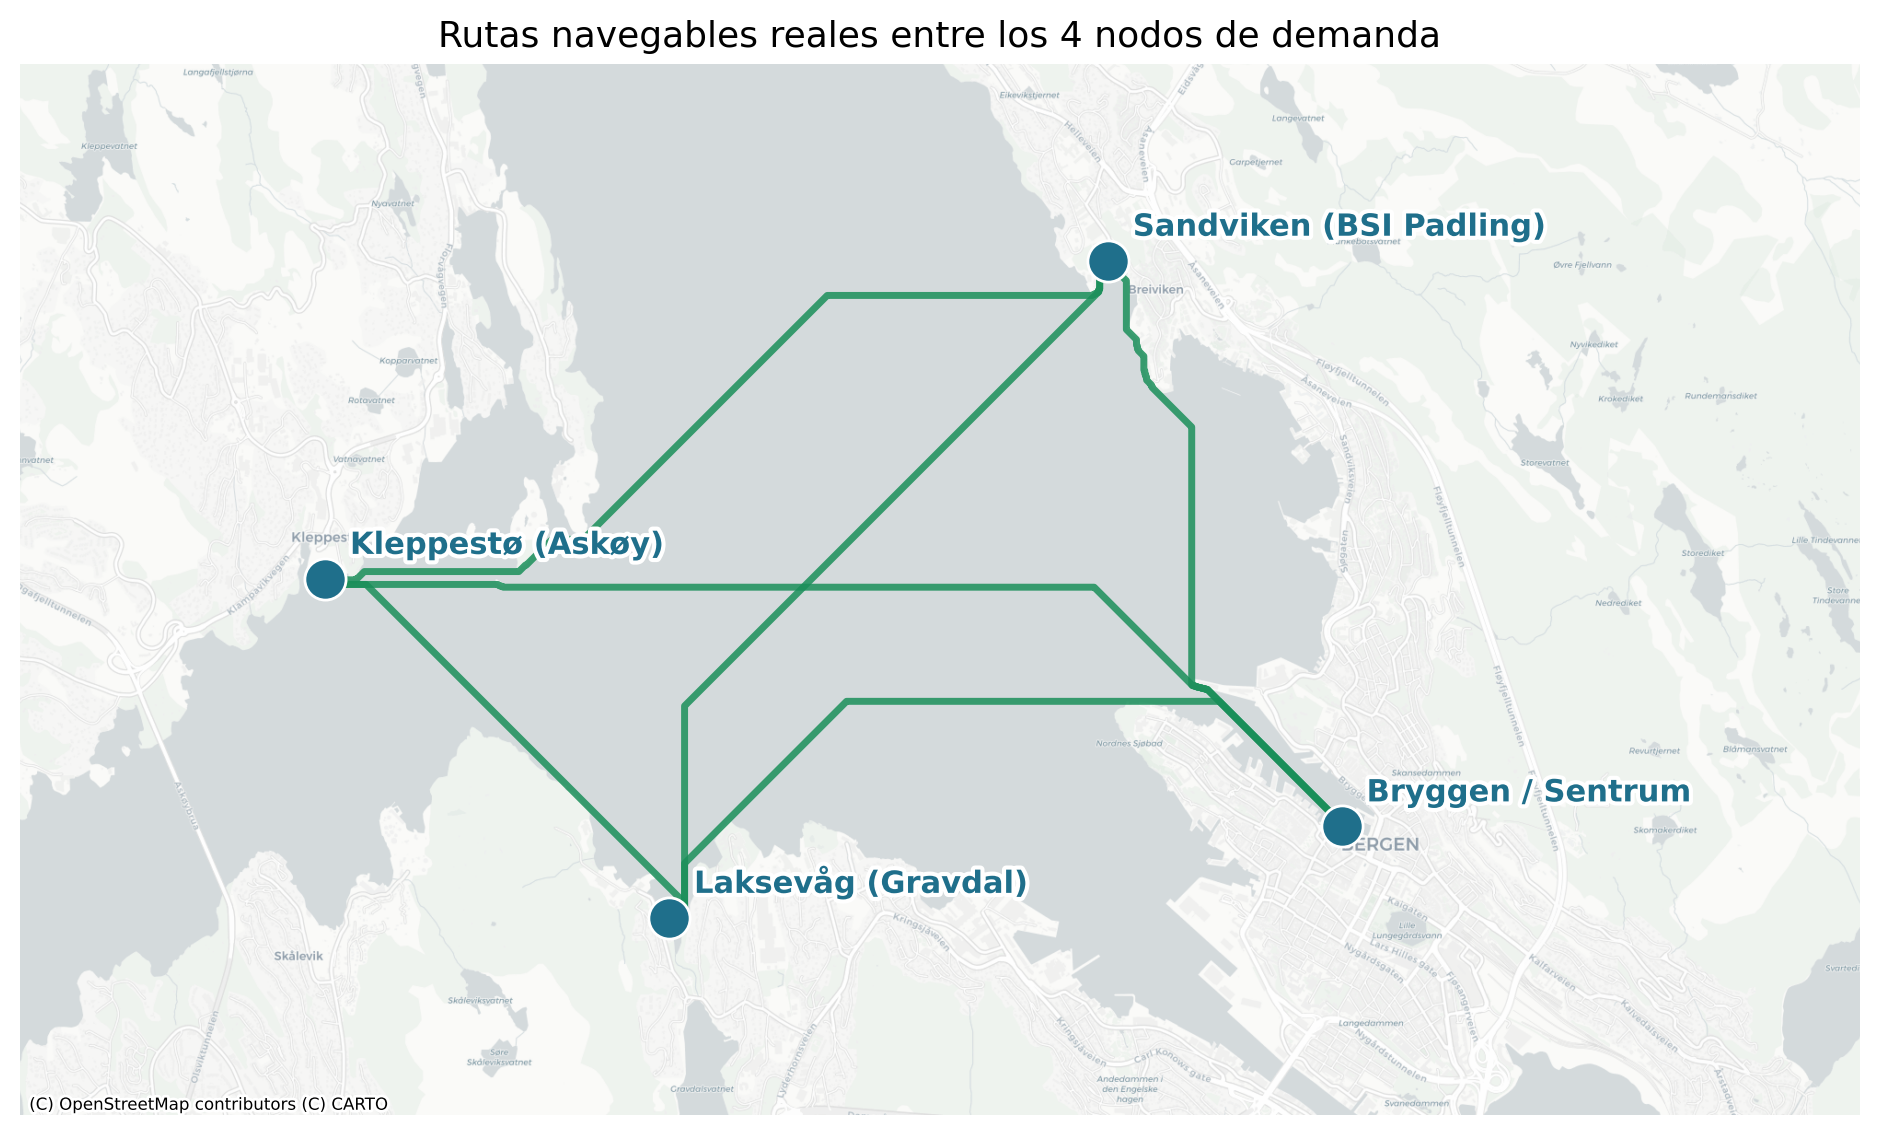
\includegraphics[width=0.75\textwidth]{figuras/mapa_rutas_navegables.png}
\caption{The six navigable routes between the four demand stops, computed by Dijkstra search over the water-classified pixel graph.}
\label{fig:mapa-rutas}
\end{figure}

The known limitation of this method is that an 8-connected grid only offers eight travel directions per step, so a shortest path can zig-zag slightly instead of following a perfect diagonal when the true direction falls between two of the eight allowed ones; the resulting overcost is a few percent in the worst case and does not affect the central conclusion that the method reliably avoids land.

% =====================================================================
\section{Demand Model}
\label{sec:demand}
% =====================================================================

No real demand data exists for this service, since it does not operate yet. Demand is therefore synthesized, but anchored in real open data wherever possible.

\subsection{Catchment areas and masses}

Population and employment are read from official Statistics Norway (SSB) 250-metre grids. For each of the four stops, a catchment area was hand-drawn by the project team in QGIS; every \emph{grunnkrets} (Norway's smallest statistical reporting unit) that the drawn area touches, even partially, is included in full for that stop, and duplicate assignments at shared boundaries are resolved by keeping each grunnkrets with the stop it overlaps the most. Population and employment are then summed over the SSB grid cells inside the resulting area. Table~\ref{tab:masas} reports the resulting masses, and Figure~\ref{fig:mapa-grunnkretser} shows which grunnkretser were assigned to each stop.

\begin{table}[H]
\centering
\caption{Catchment area, population, and employment by node (SSB grids, 2026).}
\label{tab:masas}
\begin{tabular}{lrrrr}
\toprule
Node & Grunnkretser & Area (km$^2$) & Population & Employment \\
\midrule
Kleppestø (Askøy)        & 28 & 80.6 & 25{,}153 & 7{,}550 \\
Laksevåg (Gravdal)       & 18 & 14.9 & 15{,}986 & 7{,}760 \\
Bryggen / Sentrum        & 67 & 20.2 & 27{,}695 & 52{,}213 \\
Sandviken (BSI Padling)  & 21 & 14.6 & 11{,}109 & 4{,}106 \\
\bottomrule
\end{tabular}
\end{table}

\begin{figure}[H]
\centering
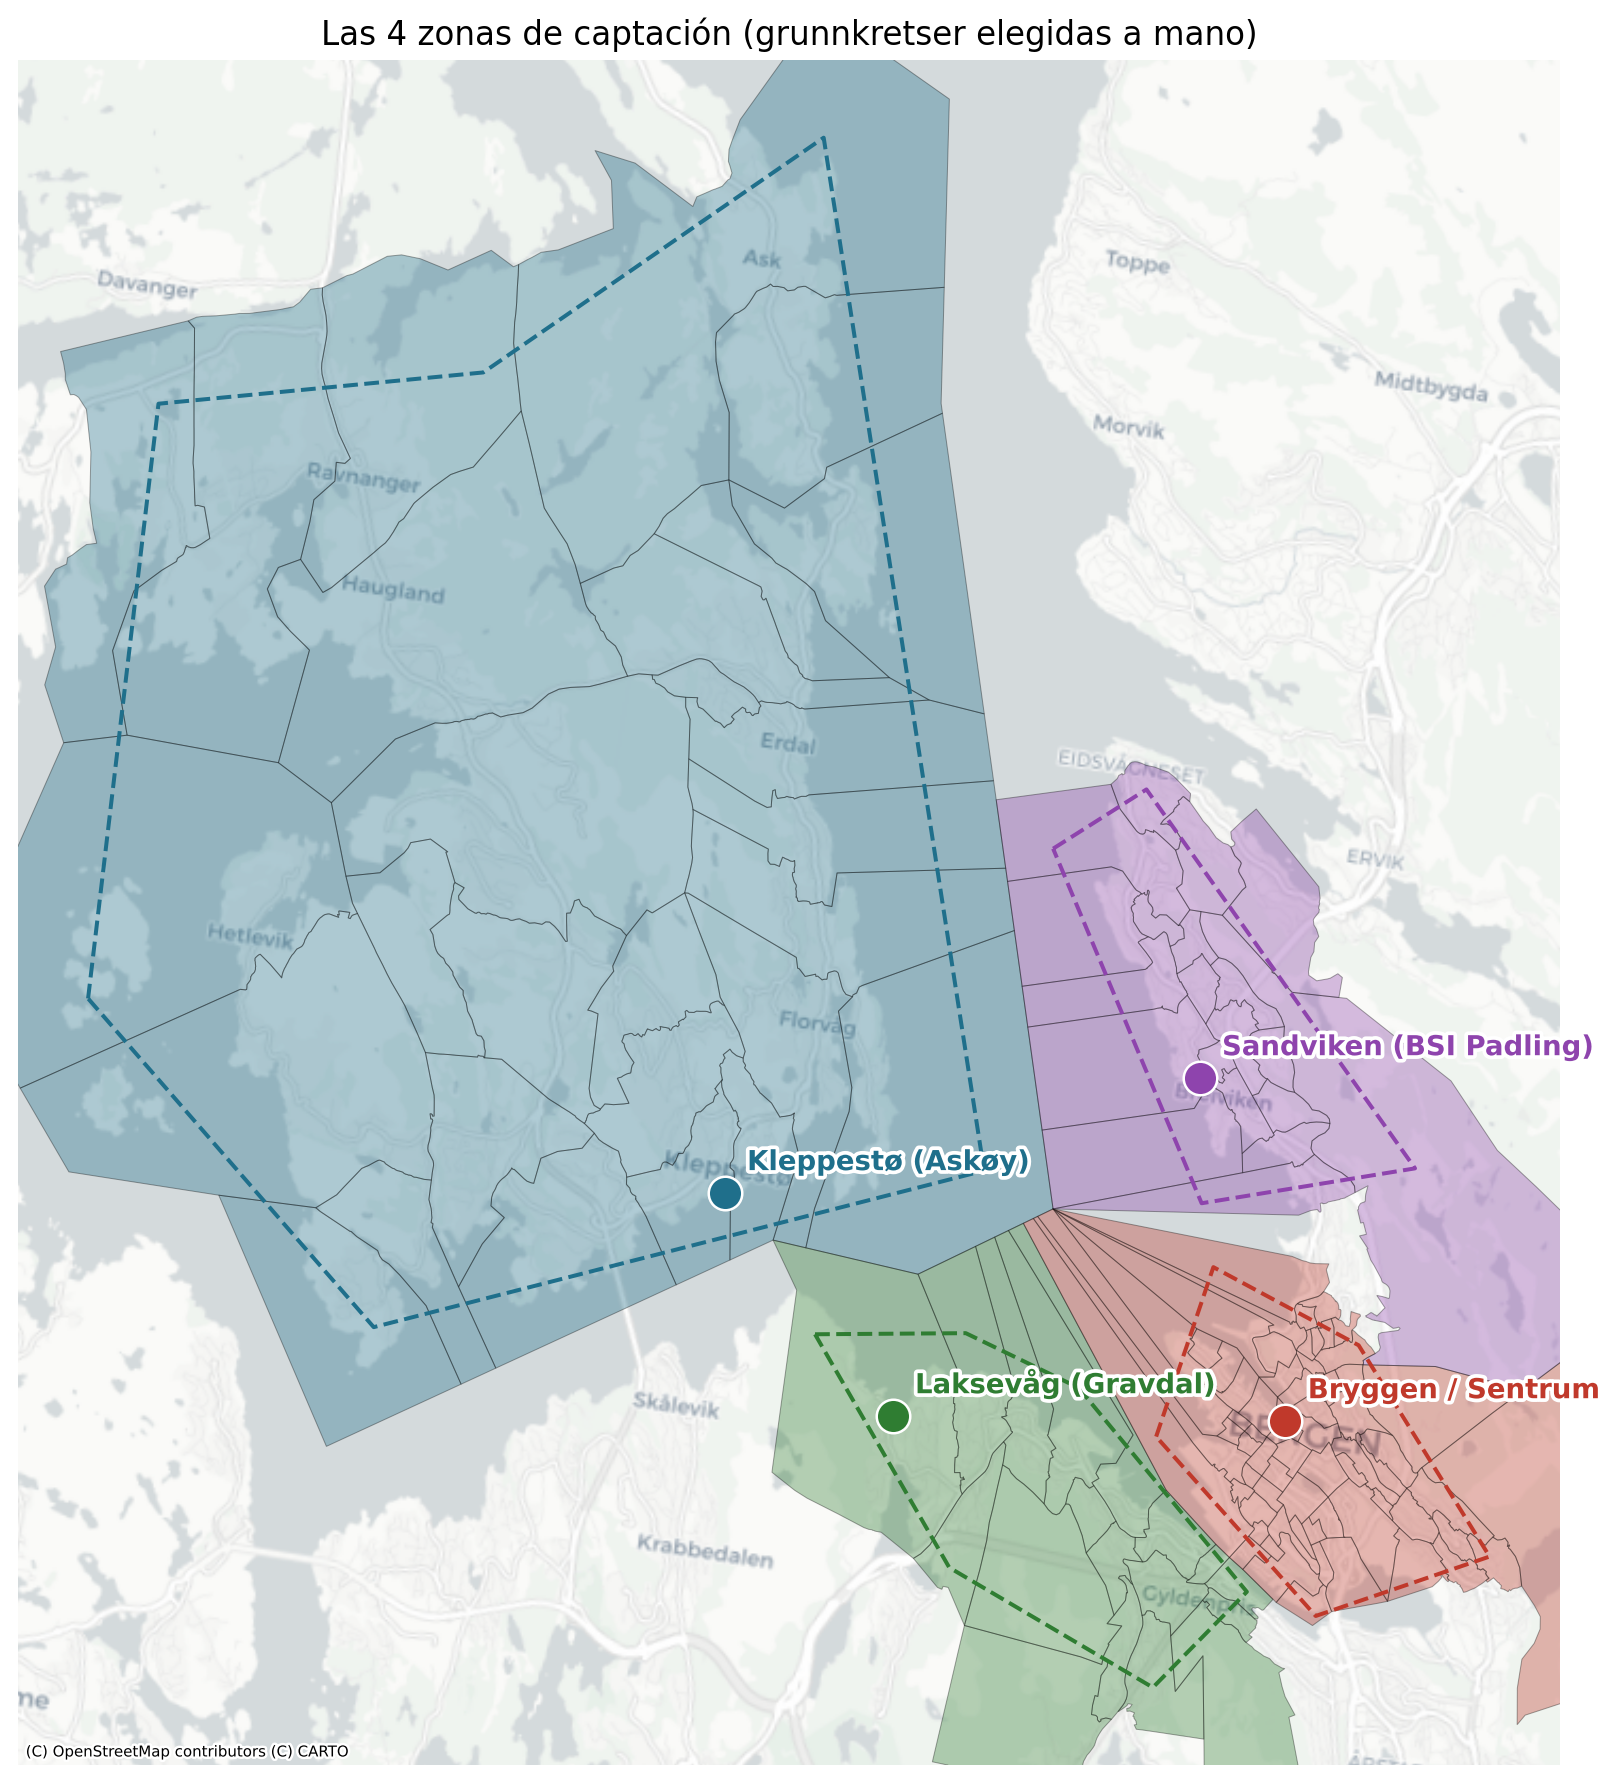
\includegraphics[width=0.85\textwidth]{figuras/mapa_general_zonas_grunnkretser.png}
\caption{The four hand-drawn catchment areas (dashed outline) and the grunnkretser assigned to each node (filled).}
\label{fig:mapa-grunnkretser}
\end{figure}

\subsection{From population and employment to origin-destination intensity}

\citet{Braathen2024} generate synthetic demand with a multiplicative popularity score,
\begin{equation}
\text{pop}_{pg} := \ln\Big(1 + \prod_{i=1}^{4} p_{i,pg}\Big),
\end{equation}
where $pg$ indexes a passenger group and the four factors $p_i$ are station-level popularity scores set by judgment for origin, destination, weekday, and hour. This project does not use that formula as written: no popularity-score table is published in the source paper to reuse, and the logarithm is specific to how that paper turns a popularity score into a deterministic group size, a step this project replaces (see below). What is adapted is the general idea of a multiplicative score built from real masses instead of judgment scores, implemented as follows.

Let $\text{pop}(n)$ and $\text{emp}(n)$ be the population and employment of node $n$ from Table~\ref{tab:masas}, and let $u(n) \in [0,1]$ be the university weighting factor described below. Masses are first normalized against the largest node, so that both scales end up comparable before being multiplied:
\begin{equation}
\text{pop}_{\text{norm}}(n) = \frac{\text{pop}(n)}{\max_m \text{pop}(m)}, \qquad
\text{emp}_{\text{norm}}(n) = \frac{\text{emp}(n)}{\max_m \text{emp}(m)} \cdot u(n).
\end{equation}
$u(n)$ compensates for the fact that registered employment does not count students, and Bergen is a university city; no open source of fine-grained enrollment data was found, so $u(n)$ is fixed by hand for now (1.0 at Bryggen and Sandviken, reduced at Kleppestø and Laksevåg), declared here as a design choice rather than measured data. A third, "mixed" mass averages the two, used at times of day with no clear commute direction:
\begin{equation}
\text{mix}(n) = \tfrac{1}{2}\big(\text{pop}_{\text{norm}}(n) + \text{emp}_{\text{norm}}(n)\big).
\end{equation}

Each of the four time bands in Table~\ref{tab:franjas} assigns a role (population, employment, or mixed) to the origin side and to the destination side of every trip; write $w(n, \text{role})$ for whichever of the three masses above that role selects. The origin-destination intensity for band $b$ and the ordered pair $(o,d)$, $o \neq d$, is then
\begin{equation}
\label{eq:intensidad}
I_b(o,d) = w\big(o, \text{role}_{\text{origin}}(b)\big) \cdot w\big(d, \text{role}_{\text{destination}}(b)\big) \cdot f_{\text{dist}}(o,d) \cdot v(b),
\end{equation}
where $v(b)$ is the band's relative volume factor (Table~\ref{tab:franjas}) and $f_{\text{dist}}$ is a distance-decay term not present in \citet{Braathen2024}'s formulation, added in this project:
\begin{equation}
f_{\text{dist}}(o,d) = \exp\!\left(-\frac{t(o,d)}{\tau}\right), \qquad \tau = 15 \text{ min},
\end{equation}
with $t(o,d)$ the navigable travel time from Table~\ref{tab:matriz-tiempos}. $I_b(o,d)$ has no unit of its own; it is a relative weight, only meaningful compared to the other 11 pairs of the same band, and is turned into an actual passenger count in the next step.

\begin{table}[H]
\centering
\caption{Time bands, relative demand volume, and origin/destination roles.}
\label{tab:franjas}
\begin{tabular}{lrll}
\toprule
Band $b$ & Hours & $v(b)$ & Role$_{\text{origin}}$ / Role$_{\text{destination}}$ \\
\midrule
Morning & 06-09 & 1.00 & population / employment \\
Midday  & 09-15 & 0.40 & mixed / mixed \\
Afternoon & 15-18 & 1.00 & employment / population \\
Evening & 18-24 & 0.15 & mixed / mixed \\
\bottomrule
\end{tabular}
\end{table}

\subsection{From intensity to Poisson arrival rates}

Every hour of the day inherits the intensity of the band it belongs to (a step function across bands, not a smoothed hourly curve): $I_h(o,d) := I_{b(h)}(o,d)$ for hour $h$ in band $b(h)$. This is computed for all 24 operating hours and all 12 ordered pairs, covering all four bands, not a subset.

The day's total passenger budget is set as a percentage of the population of the four catchment zones of Table~\ref{tab:masas} (not the total population of Bergen and Askøy), scaled down on weekends:
\begin{equation}
\label{eq:escala}
S = p \cdot P_{\text{zonas}} \cdot f_{\text{semana}}, \qquad P_{\text{zonas}} = \sum_n \text{pop}(n),
\end{equation}
where $p$ is \texttt{demanda.porcentaje\_poblacion\_dia} in the demand model's configuration file (currently 10\%, an explicit, changeable team parameter, not a value taken from either reference paper), $P_{\text{zonas}} = 79{,}943$ is the sum of the population column of Table~\ref{tab:masas}, and $f_{\text{semana}}$ is 1.0 on weekdays and 0.4 on weekends. $S$ is a number of \emph{passengers}; dividing by the mean group size $\bar{g} = 8.6$ (Section 4.4) gives the day's total number of \emph{groups}, $G = S / \bar{g}$, which is then distributed across all hour-pair cells in proportion to their share of the day's total intensity:
\begin{equation}
\lambda(o,d,h) = \frac{I_h(o,d)}{\sum_{h',o',d'} I_{h'}(o',d')} \cdot G.
\end{equation}
Within each hour, the number of arriving groups for pair $(o,d)$ is drawn $N \sim \text{Poisson}(\lambda(o,d,h))$, and each group's arrival minute is drawn uniformly within that hour.

As a reference point for the order of magnitude of $S$: \citet{Gu2021}, who study the same four stops, assume 300 travel requests per day in their case study. That number is for a water-taxi service, a different kind of offering (booked, point-to-point, presumably priced and scheduled differently from a public-transport-style service), so it is not directly comparable to $S$ here; it is mentioned only because it is a verifiable, same-instance data point, not as a validation of the 10\% figure.

\subsection{Arrivals and group sizes}

Passenger arrivals within each hour follow the Poisson process described above. \citet{Braathen2024} report a mean group size of 8.6 passengers with standard deviation 2.6, but do not specify a sampling distribution for it (their own group size is a deterministic function of the popularity score $\text{pop}_{pg}$, not a random draw). Since group size is a count of people, a discrete, non-negative distribution is used instead of a continuous one: a Binomial$(n=40, p=0.215)$, calibrated by matching moments to Braathen et al.'s reported mean and standard deviation, which reproduces the target mean exactly (8.60) and the target standard deviation closely (2.598 against 2.6).

\begin{figure}[H]
\centering
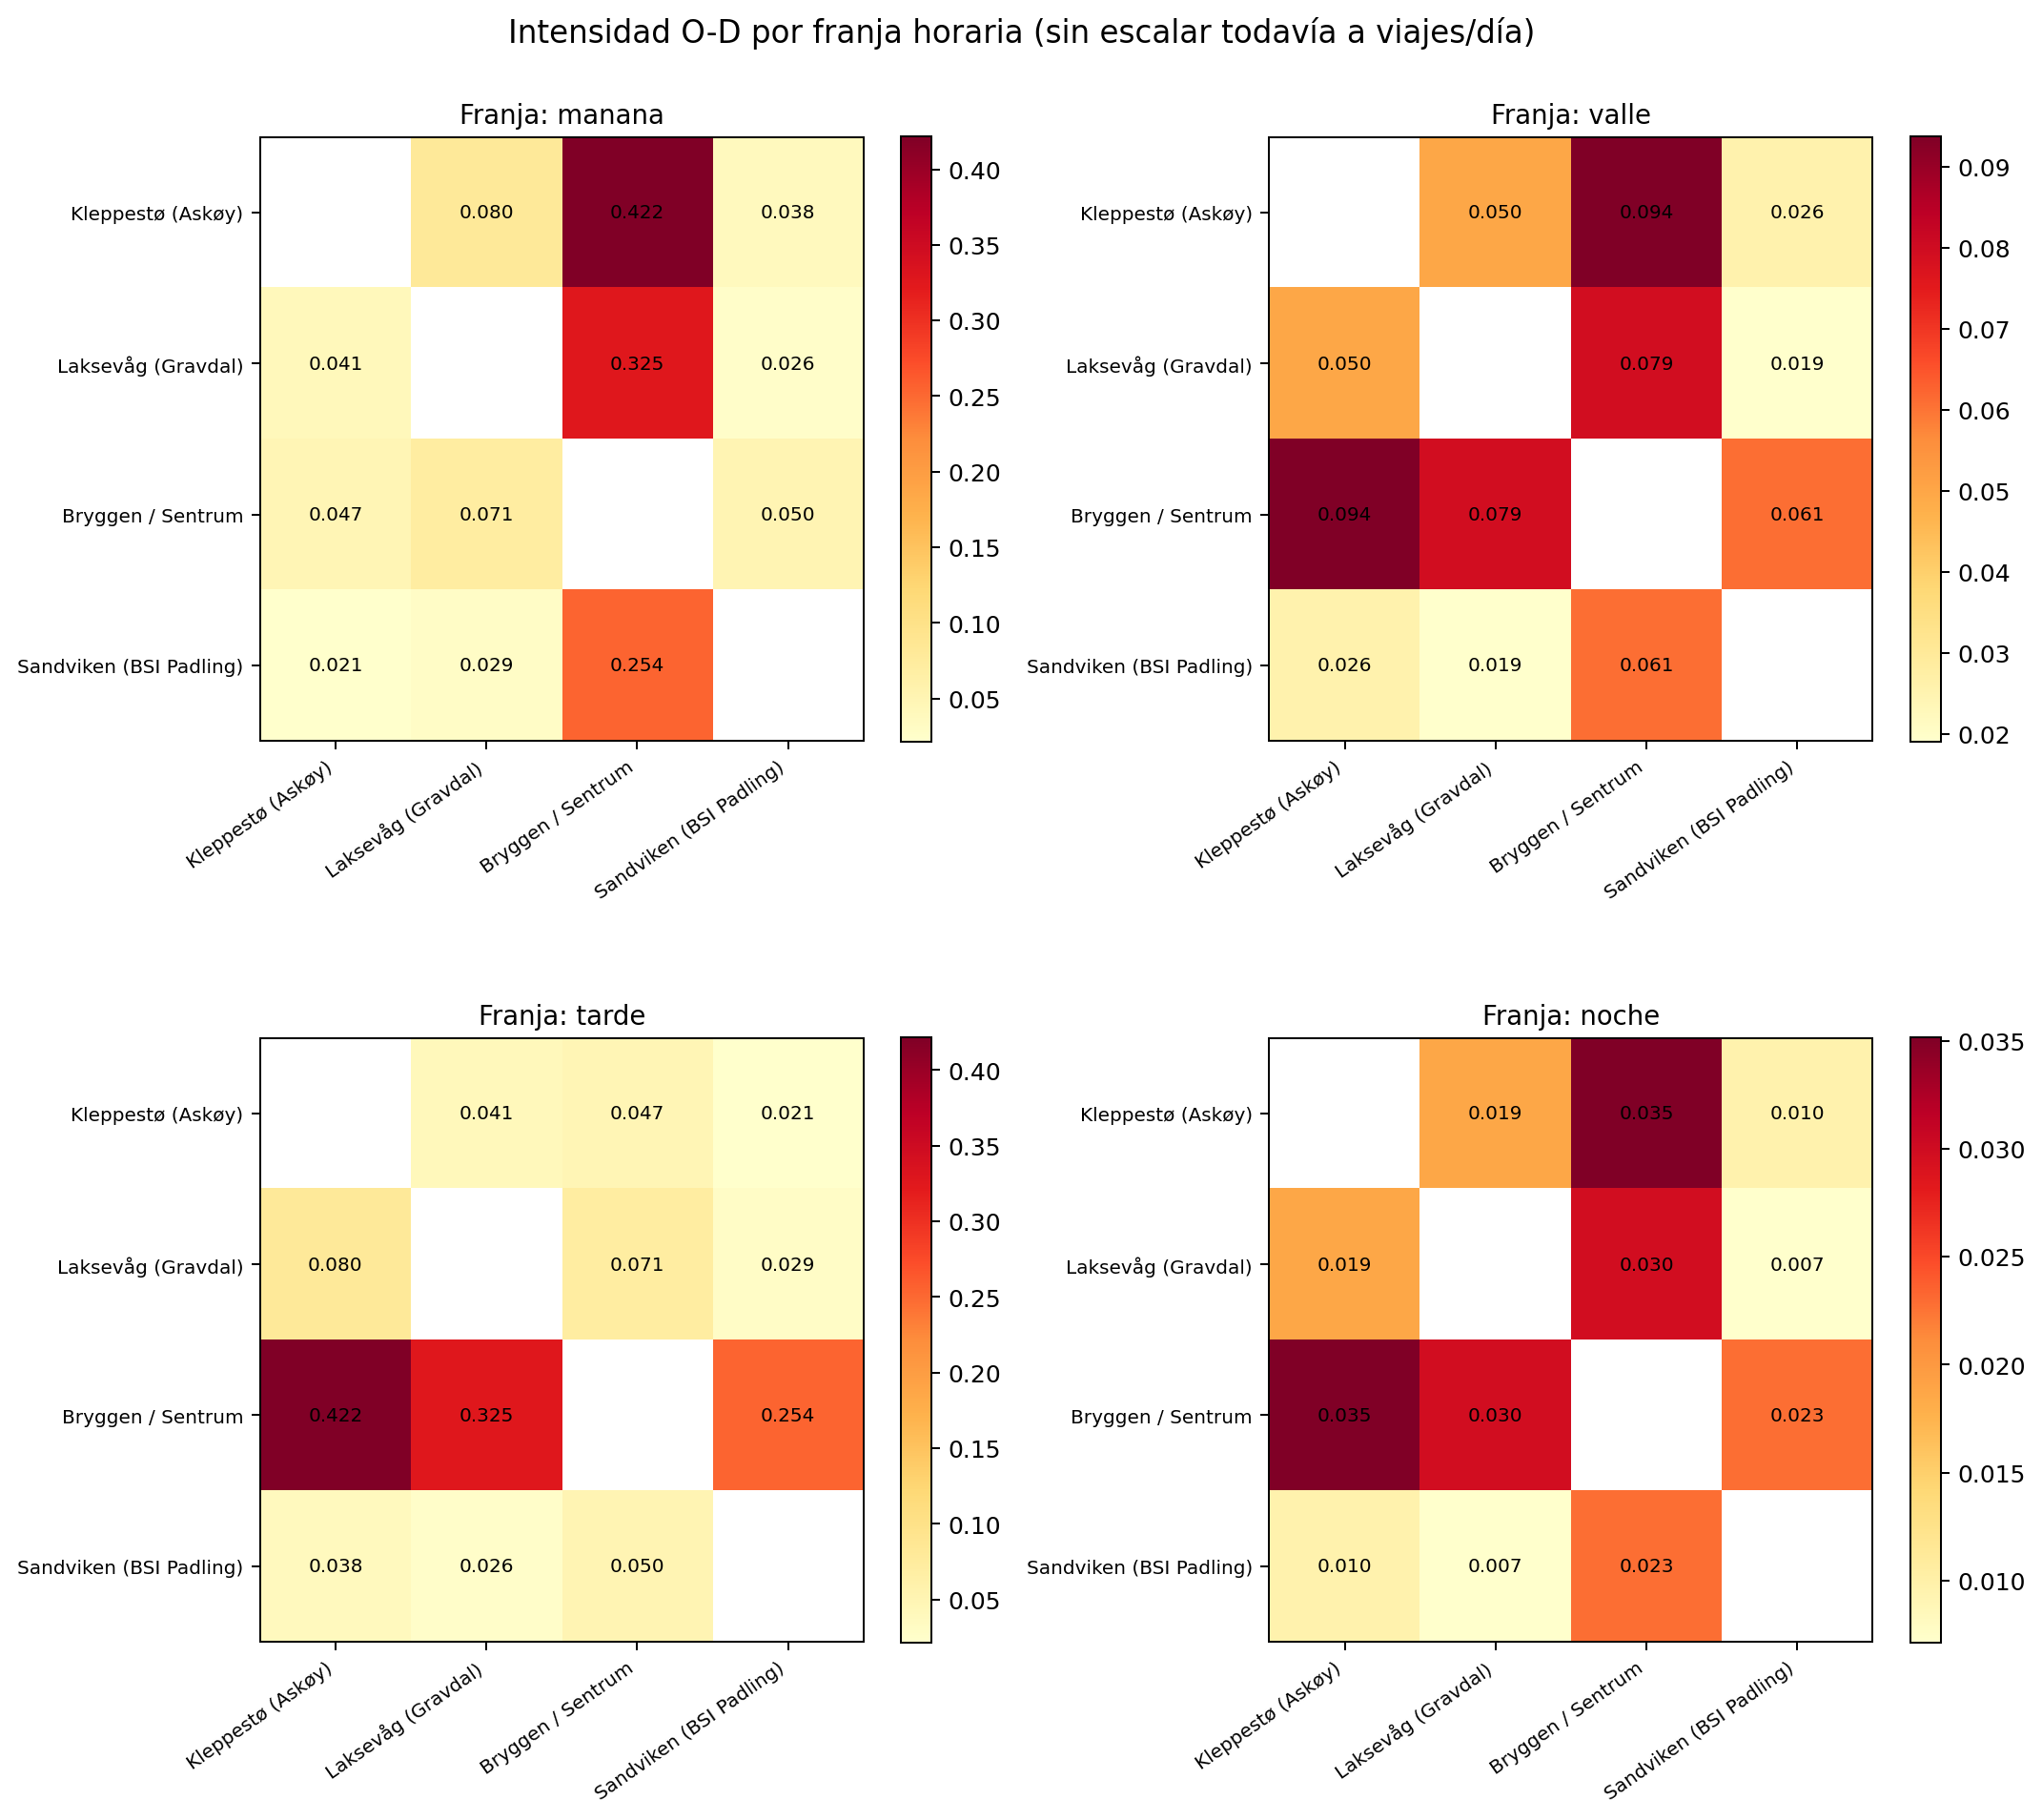
\includegraphics[width=0.85\textwidth]{figuras/heatmaps_od_por_franja.png}
\caption{Origin-destination intensity $I_b(o,d)$ by time band. Morning traffic concentrates toward Bryggen; the afternoon band reverses the pattern.}
\label{fig:heatmaps-od}
\end{figure}

\begin{figure}[H]
\centering
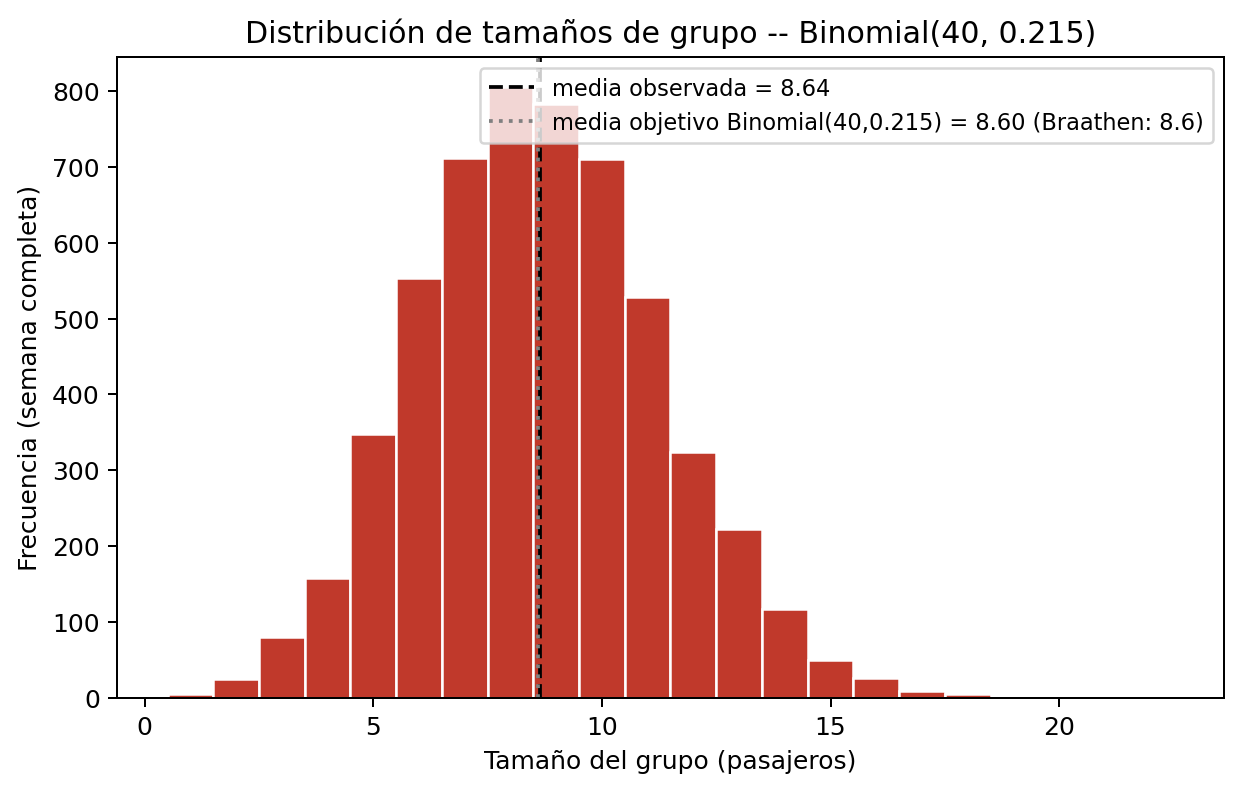
\includegraphics[width=0.7\textwidth]{figuras/histograma_tamano_grupo.png}
\caption{Observed group-size distribution over a simulated week, against the target Binomial(40, 0.215).}
\label{fig:histograma-grupo}
\end{figure}

\subsection{Persons vs.\ groups}

A group, as generated above, is the atomic unit of the demand model. For the dispatch simulation environment (Section 5), each group can optionally be exploded into individual persons, each inheriting the same origin, destination, arrival time, and patience as the group they came from; this changes the atomic unit seen by the simulator's capacity and boarding logic without altering when or where demand appears.

% =====================================================================
\section{Simulation Environment}
\label{sec:mdp}
% =====================================================================

\paragraph{This is a first, simple iteration.} The environment described in this section establishes a working structure for the dispatch problem, not the final model the project targets. It is deliberately minimal: four stops, direct point-to-point boat trips, and a small set of rules, chosen so that the environment itself (its mechanics, its bookkeeping, its interface) could be verified before adding any complexity to the model of how boats and passengers behave. Extensions are expected as the project continues.

The dispatch problem is modeled as a Markov decision process and implemented as a discrete-time simulation environment following the Gymnasium interface standard (\texttt{reset()} / \texttt{step()}), which is not a library of pre-built simulators but an interface contract: the environment implements the entire boat-and-passenger logic itself, and only its shape is standardized, so that a reinforcement-learning library can later drive it without modification. The environment advances in fixed 2-minute steps, rather than jumping between discrete events, for simplicity and because it maps directly onto the \texttt{step()} call.

\subsection{State}

The state has three parts. For each boat: origin node, destination node (equal to the origin if idle), minutes remaining until arrival, current occupancy, and whether it is free to receive a new order. For demand: one queue per origin-destination pair (twelve pairs for four nodes, not one queue per node), holding the number of people waiting and the waiting time of the oldest person in that specific pair. For time: minute of day and day of week. This rich, dictionary-shaped state is used for logging and inspection; a separate fixed-size numeric vector is derived from it for the eventual learning agent, using one-hot node encoding and cyclical (sine/cosine) time encoding so that midnight and day-of-week wraparound do not appear as artificial discontinuities to a neural network.

\subsection{Actions}

Every 2 minutes, each free boat receives one of five orders: travel to one of the four nodes, or wait. A boat already en route ignores any new order and continues to its destination; it is not redirected mid-trip. Boarding follows a fixed rule, not chosen by the policy: when a free boat at node $A$ is ordered to travel to node $B$, it boards strictly from the queue for the pair $(A,B)$, in arrival order, up to capacity, and travels directly to $B$, where everyone aboard disembarks. Trips are therefore always direct, point-to-point journeys between exactly two stops; a boat never carries passengers with mixed destinations, since it can only ever board from the one queue that matches the trip it was just ordered to make.

\subsection{Transition}

Each step executes, in order: (1) apply the chosen action to every free boat, boarding from the matching pair queue as described above; (2) advance all boats in transit by the fixed time step, disembarking everyone aboard any boat that reaches its destination; (3) add to the queues any new arrivals whose arrival time falls within the interval just elapsed (these do not board the boat that just departed in step 1, since they had not yet arrived when boarding happened); (4) remove, as lost, any waiting person whose patience has been exceeded; (5) compute the step's reward and assemble the new state.

\subsection{Reward}

The reward is negative (a sum of penalties) and combines three terms, computed every 2 minutes:
\begin{equation}
\text{surplus} = \max(0,\ \text{time in system} - \tau_{\text{tol}}), \qquad
\text{surplus}_{\max} = \max(\varepsilon,\ \text{patience} - \tau_{\text{tol}}),
\end{equation}
\begin{equation}
r = -\Bigg[ \sum_{\text{active persons}} \left(\frac{\text{surplus}}{\text{surplus}_{\max}}\right)^{2}
\ +\ P_{\text{lost}} \cdot (\text{persons lost this step})
\ +\ w_{\text{move}} \cdot (\text{boats under way this step}) \Bigg],
\end{equation}
with tolerance $\tau_{\text{tol}} = 12$ minutes (the longest direct navigable route, from Table~\ref{tab:matriz-tiempos}), loss penalty $P_{\text{lost}} = 1.3$, and movement penalty $w_{\text{move}} = 0.1$; all three parameters live in the environment's configuration file, not hard-coded.

To see the magnitude of each term concretely: a person still waiting exactly at the 12-minute tolerance contributes 0 (inside the free zone); a person about to be lost (surplus close to $\text{surplus}_{\max}$) contributes close to 1; ten such people near their limit at the same step therefore contribute close to $-10$ to $r$. A single lost person costs $P_{\text{lost}} = 1.3$, deliberately set a little above 1 so that losing someone is always somewhat worse, in the reward, than leaving them waiting at the very edge of their patience. A boat moving costs only $0.1$, small on purpose so that the model is not discouraged from dispatching boats when doing so is actually needed. The penalty grows quadratically in the surplus ratio, so it stays small while a person is only moderately over the tolerance and accelerates as they approach their patience limit, which is meant to weight attention toward the passengers closest to being lost rather than spreading pressure evenly.

One gap in this formula was found and closed while implementing it: patience on strong connections is 15 minutes with random jitter of $\pm 5$ minutes (already part of the demand generator), so it can fall as low as 10 minutes, below the 12-minute tolerance, which would make $\text{surplus}_{\max}$ zero or negative for those cases. This is corrected with the floor $\varepsilon = 1.0$ minute shown above: for the rare cases this affects, the penalty simply saturates near its maximum almost immediately. The demand generator and its jitter were left untouched; the correction lives entirely in the reward function.

\bibliographystyle{plainnat}
\bibliography{referencias}

\end{document}
